%!TEX root = ../Electrodynamics.tex

\subsection{Граничные условия для поперечных волновых функций волн ТЕ, ТМ, ТЕМ типов в идеальной линии передачи. Математическая формулировка задачи описания волн ТЕ, ТМ, ТЕМ типов.}
\begin{figure}[h!]
  \centering
  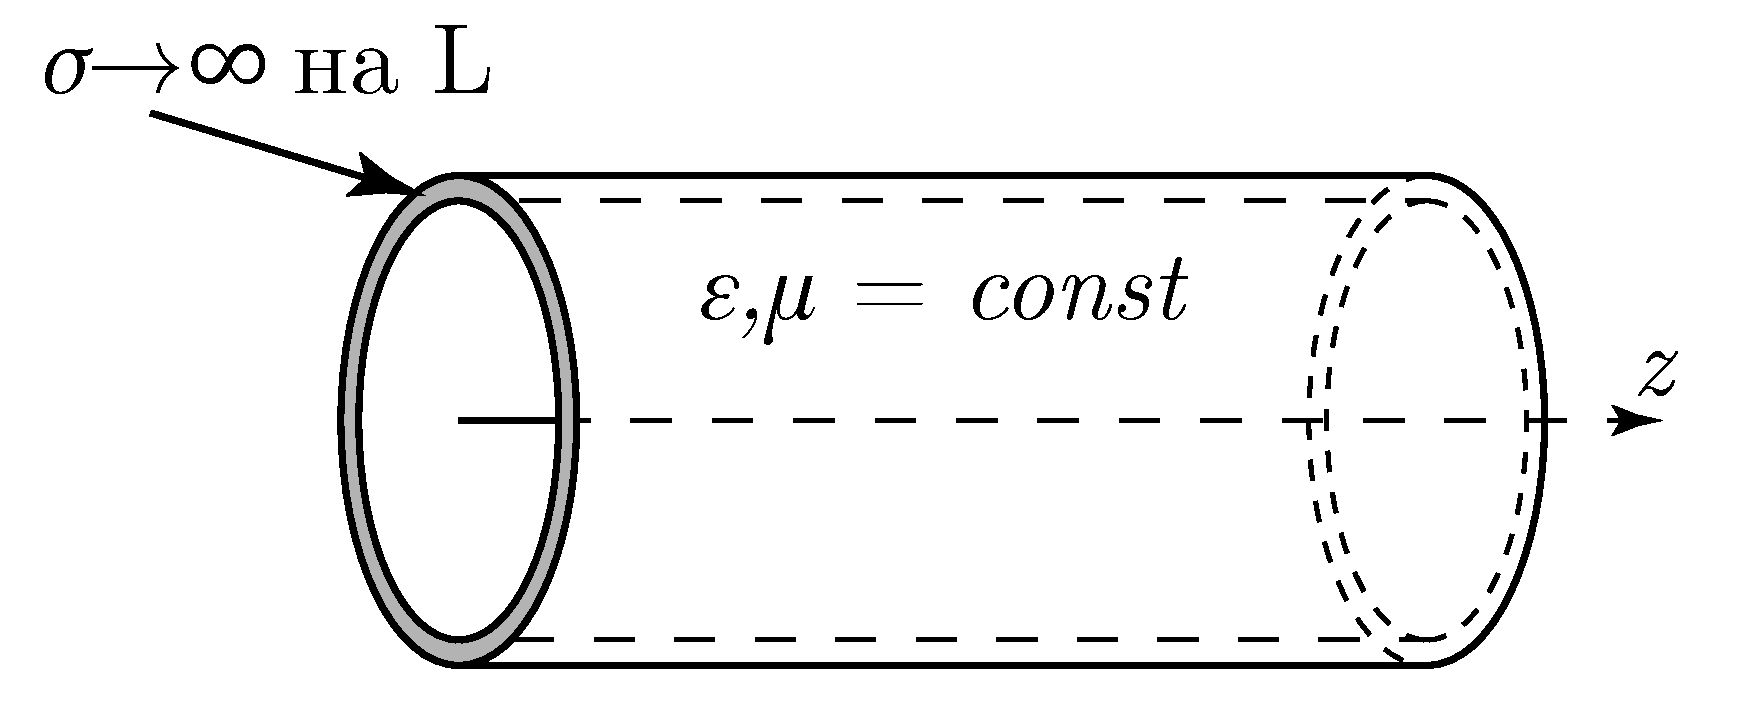
\includegraphics[width = 0.6\linewidth]{img/t21.pdf}
\end{figure}
Рассмотрим случай идеального проводника, $\sigma \rightarrow \infty$(Вообще говоря, идеальных проводников не бывает,
однако условие идеальной проводимости можно записать в виде: $\sigma \gg w ~(\delta \ll L)$ ).
Вспомним граничные условия для полей на поверхности идеального проводника:
\begin{equation}
  E_{\tau}|_S = 0,~H_n|_S = 0,
\end{equation}
а также условие на поперечную волновую функцию:
\begin{equation}
  \Delta_{\perp}\psi^{e,m}+\varkappa^2\psi^{e,m}=0
\end{equation}
Найдем граничные условия для $\psi^{e,m}$ для идеальной ЛП.

\textbf{ТМ-волна}:
\begin{equation}
  \text{т.к. }E_z \sim \psi^e,~\vec{E}_{\perp \tau}\sim \frac{\partial \psi^e}{\partial \tau} 
\end{equation}
\begin{equation}
  \text{и }E_z = 0,~E_{\perp \tau} = 0 
\end{equation}
\begin{equation}
  \text{то }\psi^{e}(\vec{r}_{\perp})|_S = 0
\end{equation}
- это граничное условие Дирихле

\textbf{ТЕ-волна}:
\begin{equation}
  \text{т.к. }\vec{E}_{\perp \tau}\sim [\nabla_{\perp} \psi^m(\vec{r}_{\perp})\times\vec{z_0}]_{\tau} 
\end{equation}
\begin{equation}
  \text{и }E_{\perp \tau} = 0 
\end{equation}
\begin{equation}
  \text{то }\frac{\partial \psi^m}{\partial n}|_S = 0
\end{equation}

\textbf{ТЕМ-волна}:
\begin{equation}
  \text{т.к. }\vec{E}_{\perp \tau}\sim \nabla_{\perp} \psi^m(\vec{r}_{\perp}) 
\end{equation}

\begin{equation}
  \text{то }\frac{\partial \psi}{\partial \tau}|_S = 0 \Rightarrow \psi|_S = const = C_i
\end{equation}

Отметим, что на разных поверхностях проводников постоянная $C_i$ может быть разной.

\textbf{Математическая формулировка задач для описания волн.}

\textbf{ТМ}. Необходимо решить:
\begin{align*}
  &\Delta_{\perp}\psi^{e}+\varkappa^2\psi^{e}=0\\
  &\psi^e|_L = 0 , \text{$L$ - граничный контур}
\end{align*}

\textbf{ТЕ}. Необходимо решить:
\begin{align*}
  &\Delta_{\perp}\psi^{m}+\varkappa^2\psi^{m}=0\\
  &\frac{\partial \psi^m}{\partial n}|_L = 0
\end{align*}

\textbf{ТЕМ}. Необходимо решить:
\begin{align*}
  &\Delta_{\perp}\psi^{m}=0\\
  &\psi|_{L_i} = C_i
\end{align*}
Задачи ТЕ, ТМ волн - аналогичны задачам с мембраной, где граница мембраны закреплена неподвижно, а ТЕМ задачу можно
назвать <<электростатической>>.
Это задачи на нахождение собственных функций
\begin{equation}
  \psi^{e,m}_1(\vec{r}_{\perp}),\psi^{e,m}_2(\vec{r}_{\perp}),\dots \psi^{e,m}_i(\vec{r}_{\perp})      
\end{equation}
и собственных чисел 
\begin{equation}
\varkappa_1,\varkappa_2,\dots,\varkappa_i  
\end{equation}
Если ЛП идеальна, то спектр сбственных значений и функций бесконечен.